\section{Salut Vazaha}

21 nov. 2010

\begin{multicols}{2}

Salut tout le monde, voici les premières nouvelles de mon voyage qui se déroule idéalement pour le moment, malgré les problèmes politiques qui ont pu vous être rapportés par les infos internationales. A Madagascar, la politique est surtout une histoire de politiciens de la capitale, les gens suivent cela de loin sans considérer que ça puisse changer quoi que ce soit dans leur vie. En fait il semble vraiment que la tentative de putsch soit une affaire de militaires pour laquelle mêmes les habitants de Tana ne se sentent pas vraiment concernés. Un certain fatalisme règne. En fait, le point qui me concerne est l'aéroport d'Ivato, seule aéroport de la capitale, qui semble avoir été bloqué quelques heures, affaire à suivre.

Je suis arrivé à Ivato (extérieur de Tana) dimanche matin et me suis directement dirigé vers la ville en taxi brousse, l'occasion de se faire la main avec la monnaie locale. L'Ariary utilisé actuellement vaut 5 francs malgache. Même si l'ariary a remplacé officiellement le FMG en 2005, bon nombre de personnes parlent encore en FMG, soit pour tromper le touriste, soit par habitude.

Dans Tana, je me suis balladé avec le sac sur le dos avant de me poser dans un parc pour regarder jouer au foot des jeunes et admirer la ville.

%<img src="http://etienne.croclemonde.org/public/madagascar/DSCF0110.JPG" />
%<img src="http://etienne.croclemonde.org/public/madagascar/DSCF0116.JPG" />

Le lendemain j'ai pris un taxi brousse pour Antsirabe, à 3 heures au sud, sur la RN7, bonne route goudronnée. A Antsirabe, "capitale du pousse pousse", la découverte des environs est au programme, j'ai alors loué un vélo pour aller faire une boucle d'une quinzaine de kilomètres dans la campagne voisine avec pour cible un lac des environs.

%<img src="http://etienne.croclemonde.org/public/madagascar/DSCF0126.JPG" />
%<img src="http://etienne.croclemonde.org/public/madagascar/DSCF0132.JPG" />

Je me suis alors posé pour discuter avec des enfants, tout étonnés de voir un vazaha ici et super contents de se voir sur le petit écran de l'appareil photo.

%<img src="http://etienne.croclemonde.org/public/madagascar/DSCF0139.JPG" />

Puis le lendemain direction le sud toujours, halte à Fianarantsoa avant de prendre l'unique train de l'île, vers Manakar. Je me promène dans la ville et visite les marchés, mon but est d'aller me perdre dans les ruelles, j'étonne alors tout le monde car ce n'est pas une place où les touristes vont en général. Voici une photo prise en montée raide près du marché.

\smallbreak
\hspace*{-0.65cm}
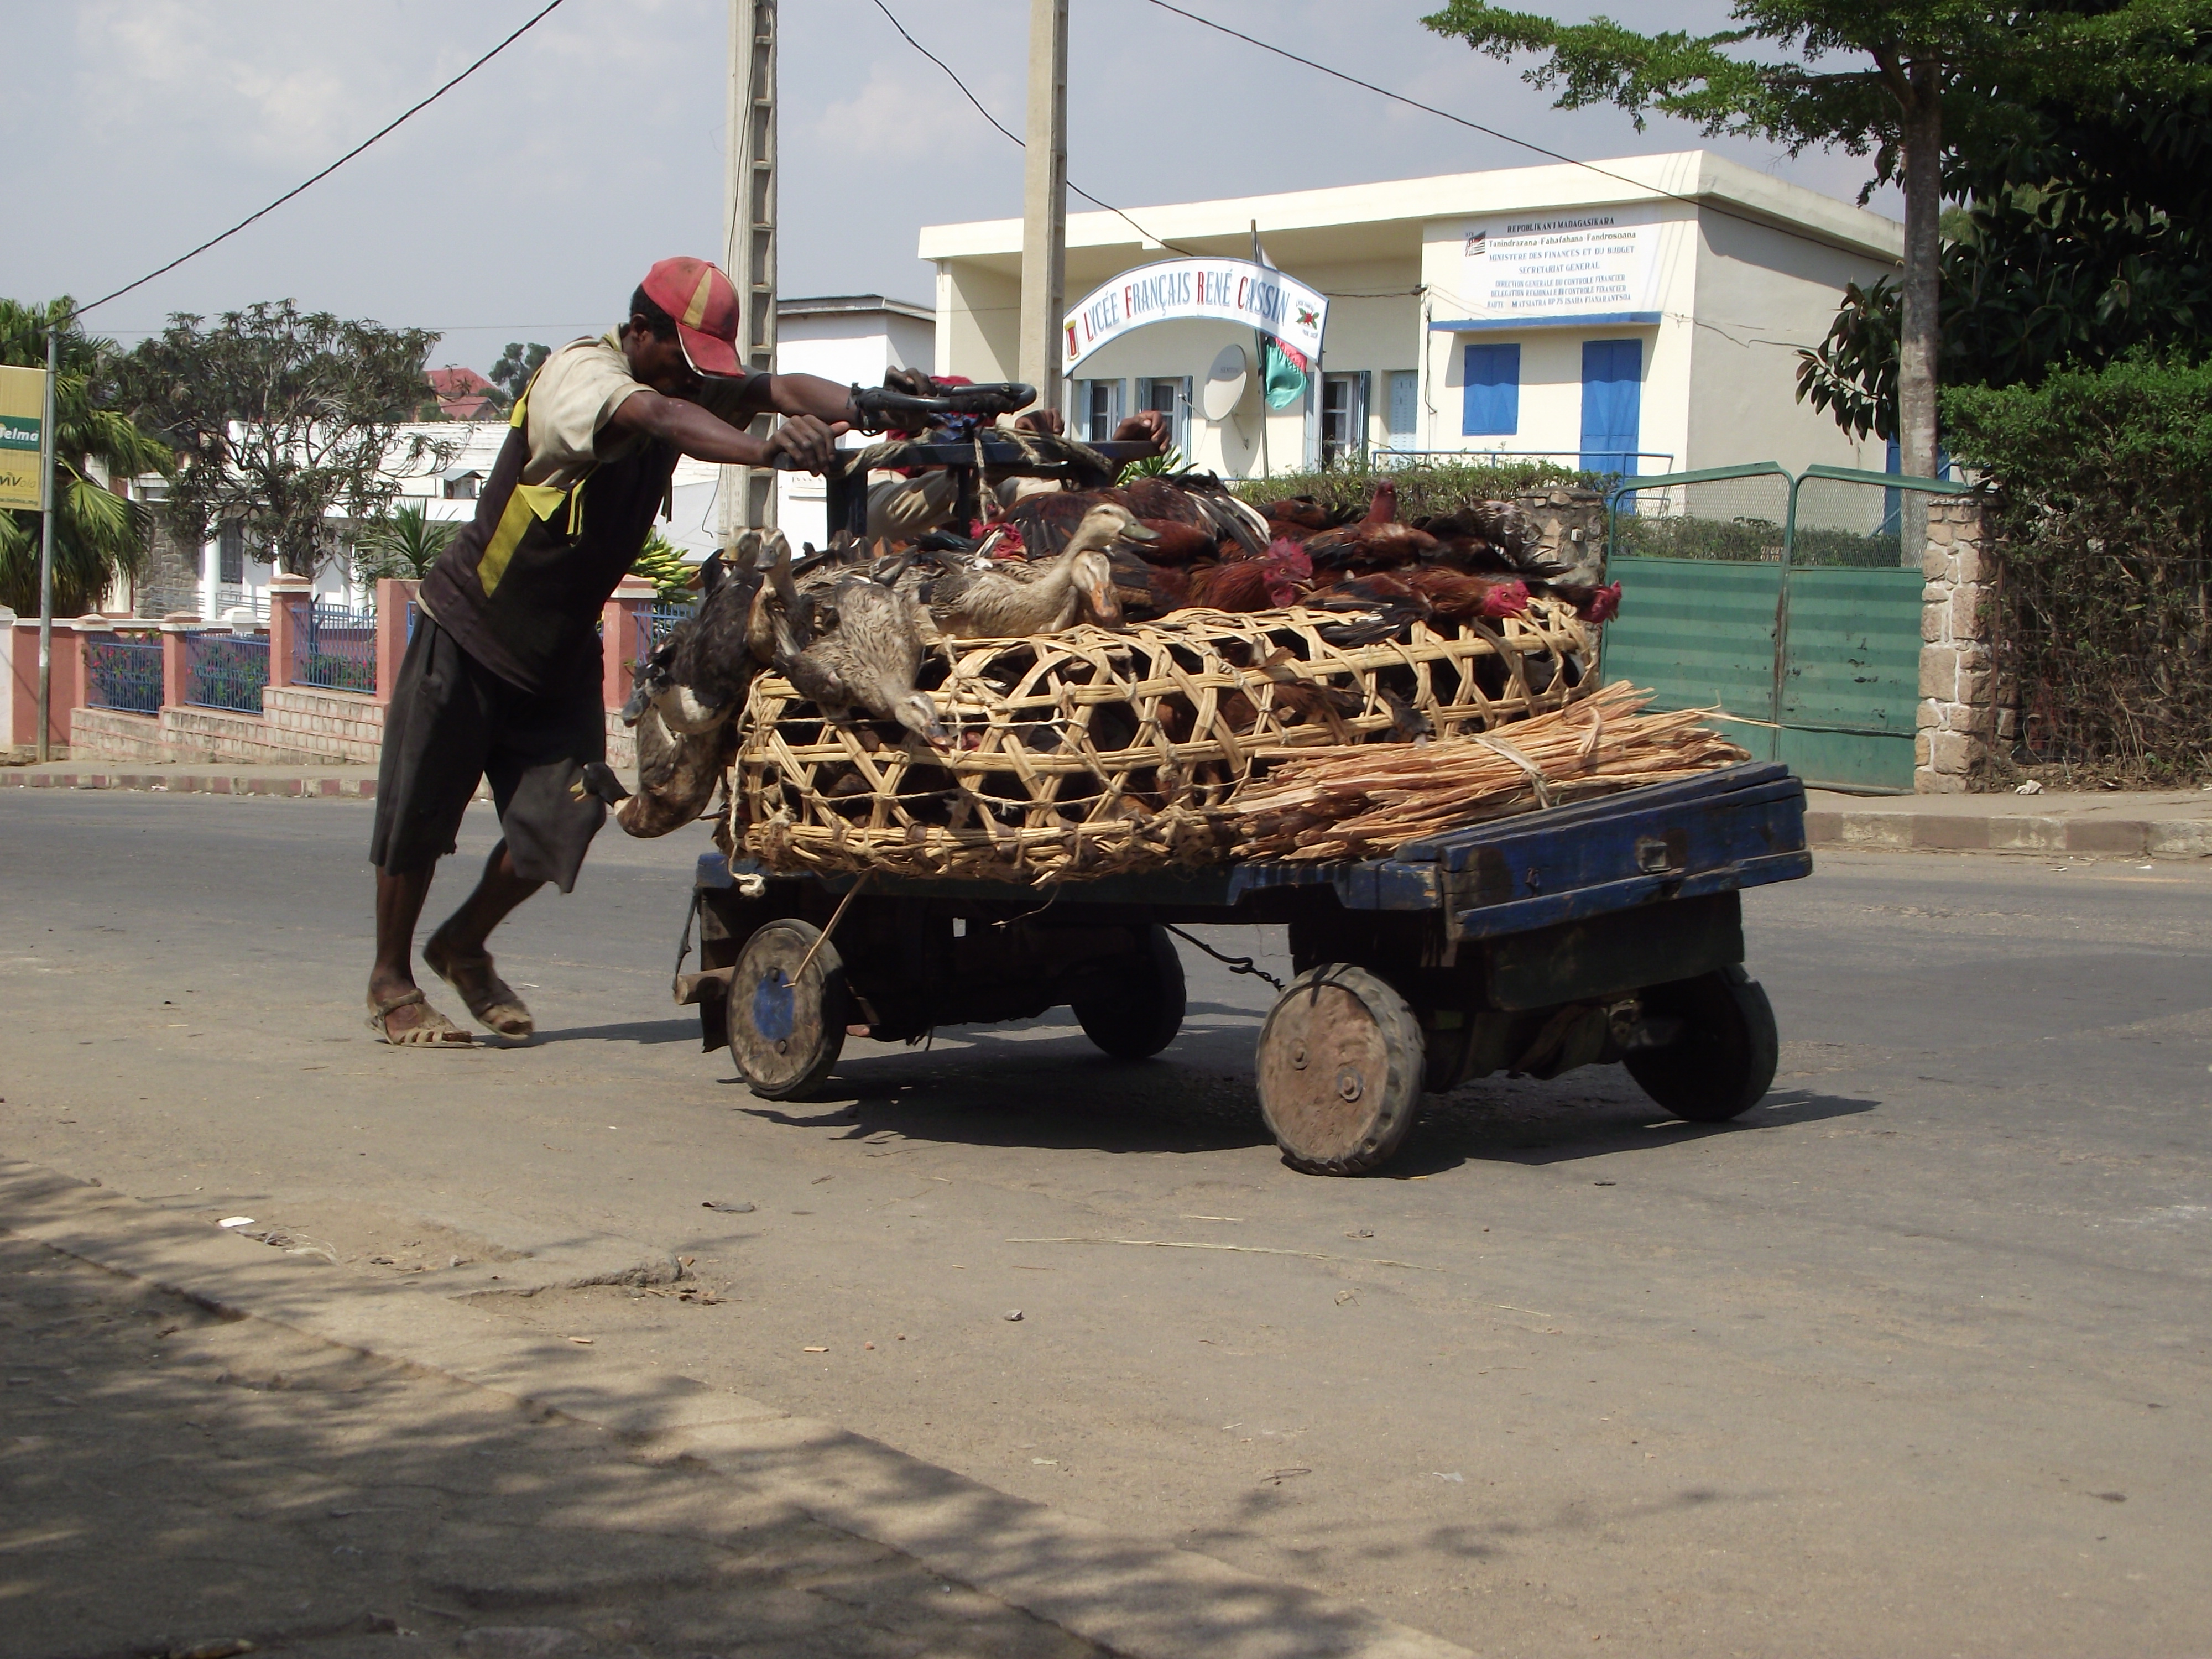
\includegraphics[width=5cm]{articles/Salut-vazaha/DSCF0151.JPG}
\smallbreak

Puis j'ai pris le train vers Manakar. Ce train est décrit par beaucoup comme LE moment inoubliable de la visite de l'île, grosse attente de ma part donc. Sur un peu moins de 200 km vers la côte, nous avons alors traversé des paysages magnifiques, allant des rizières aux plantations de thé, des bananiers à la traversée des villages que ce train permet de désenclaver. Durant toute cette traversée et durant le séjour à Manakar, je suis resté avec Mélanie et Grégoire, deux voyageurs qui rentrent bientôt en France. Ayant les mêmes méthodes de voyage, nous nous sommes très bien entendu.

%<img src="http://etienne.croclemonde.org/public/madagascar/DSCF0175.JPG}
\smallbreak

\smallbreak
\hspace*{-0.65cm}
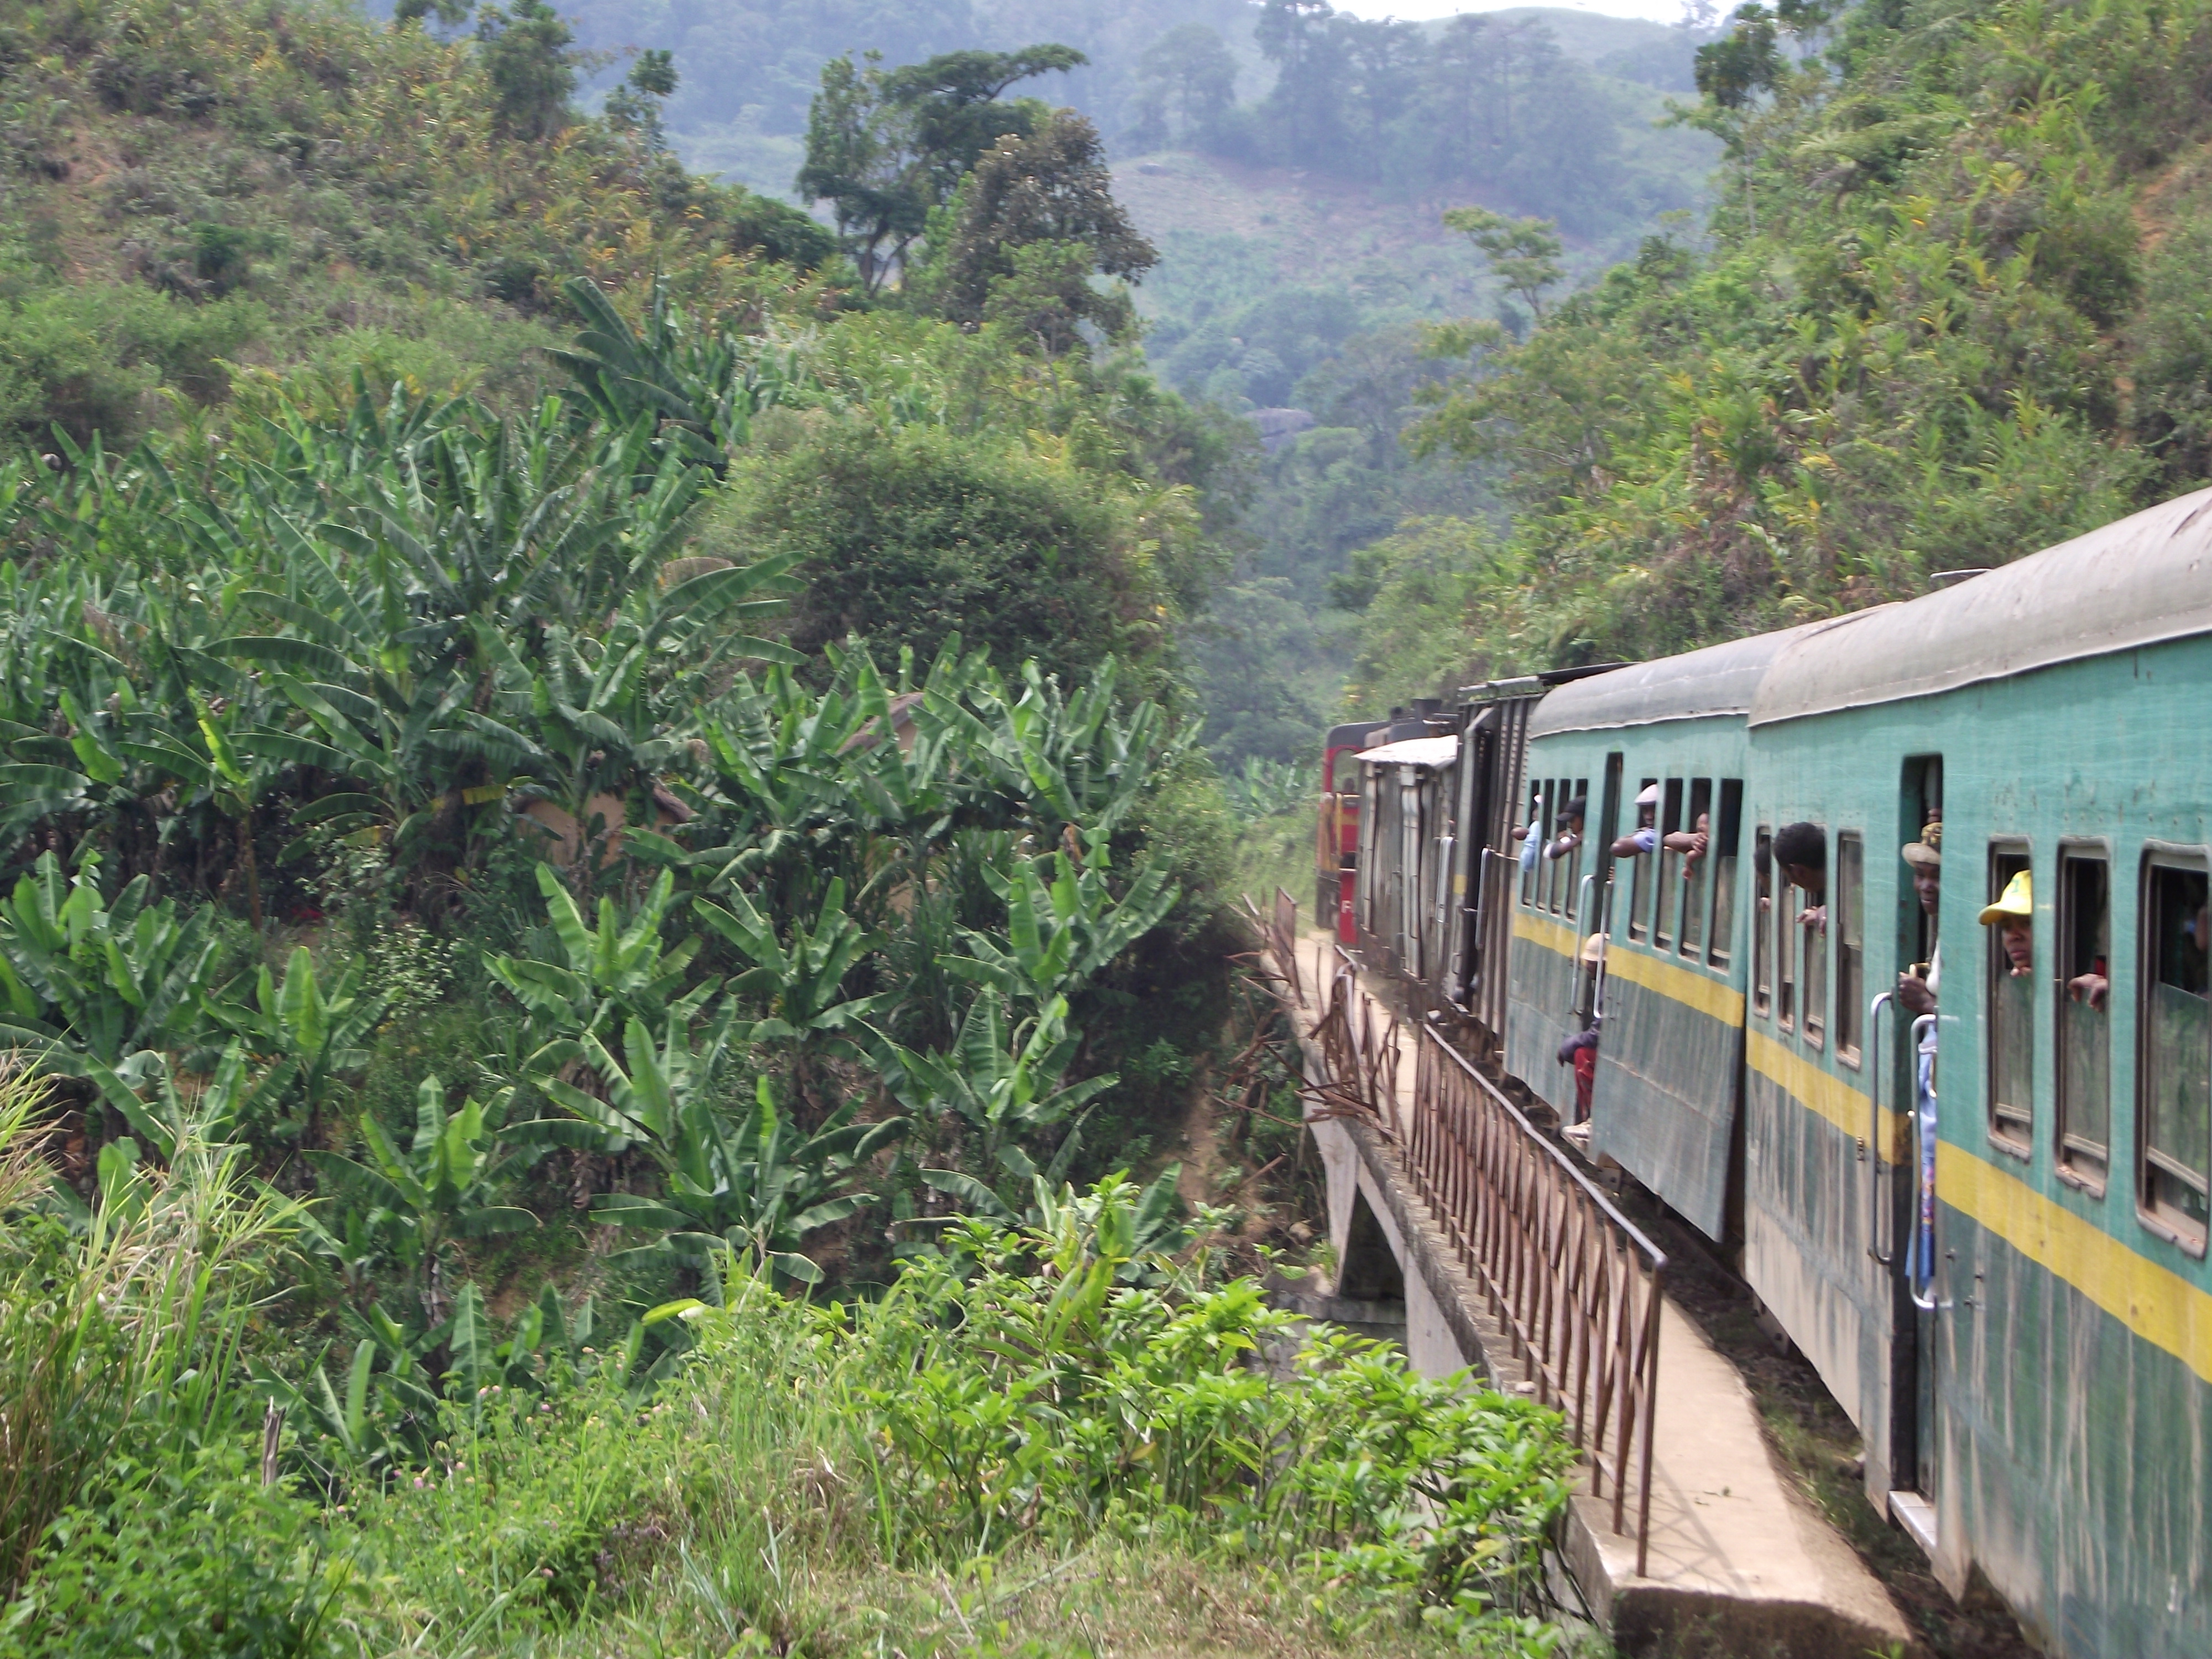
\includegraphics[width=5cm]{articles/Salut-vazaha/DSCF0196.JPG}
\smallbreak

\smallbreak
\hspace*{-0.65cm}
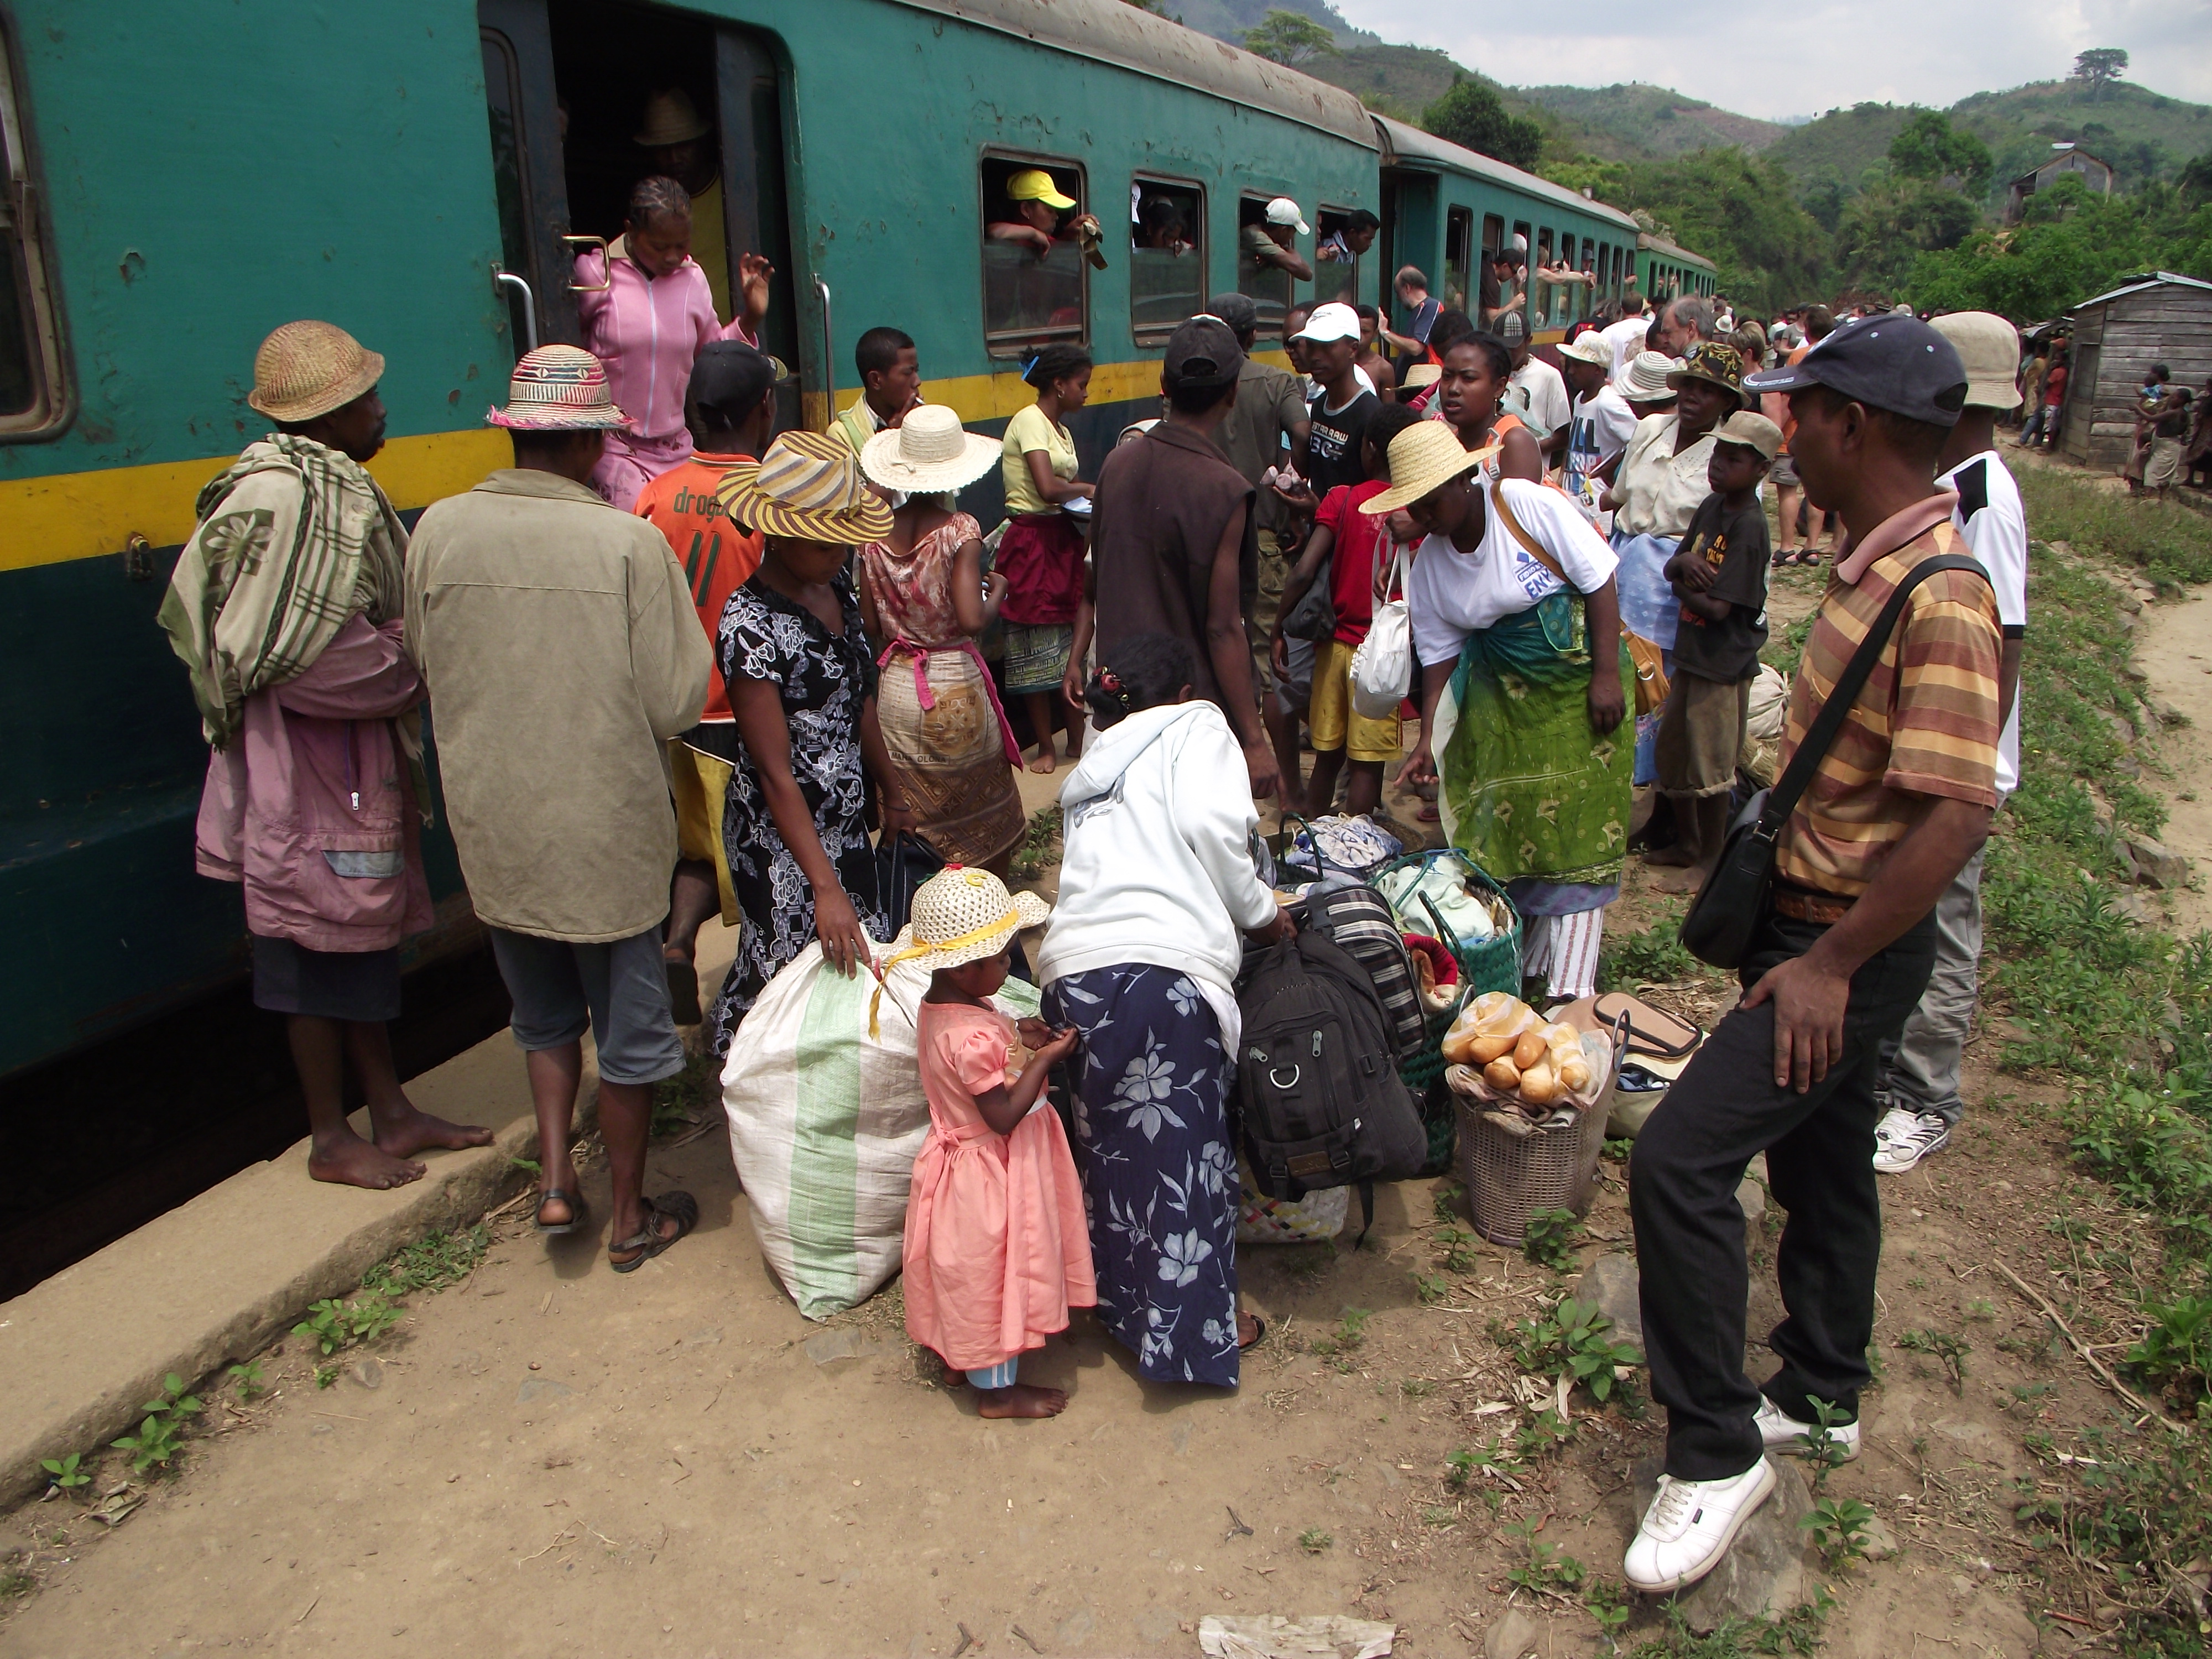
\includegraphics[width=5cm]{articles/Salut-vazaha/DSCF0197.jpg}
\smallbreak

Puis dans Manakar, nous avons fait une petite visite sur le canal, creusé pour permettre le transport de marchandises sans passer par la mer, très dangereuse sur cette côte.

\smallbreak
\hspace*{-0.65cm}
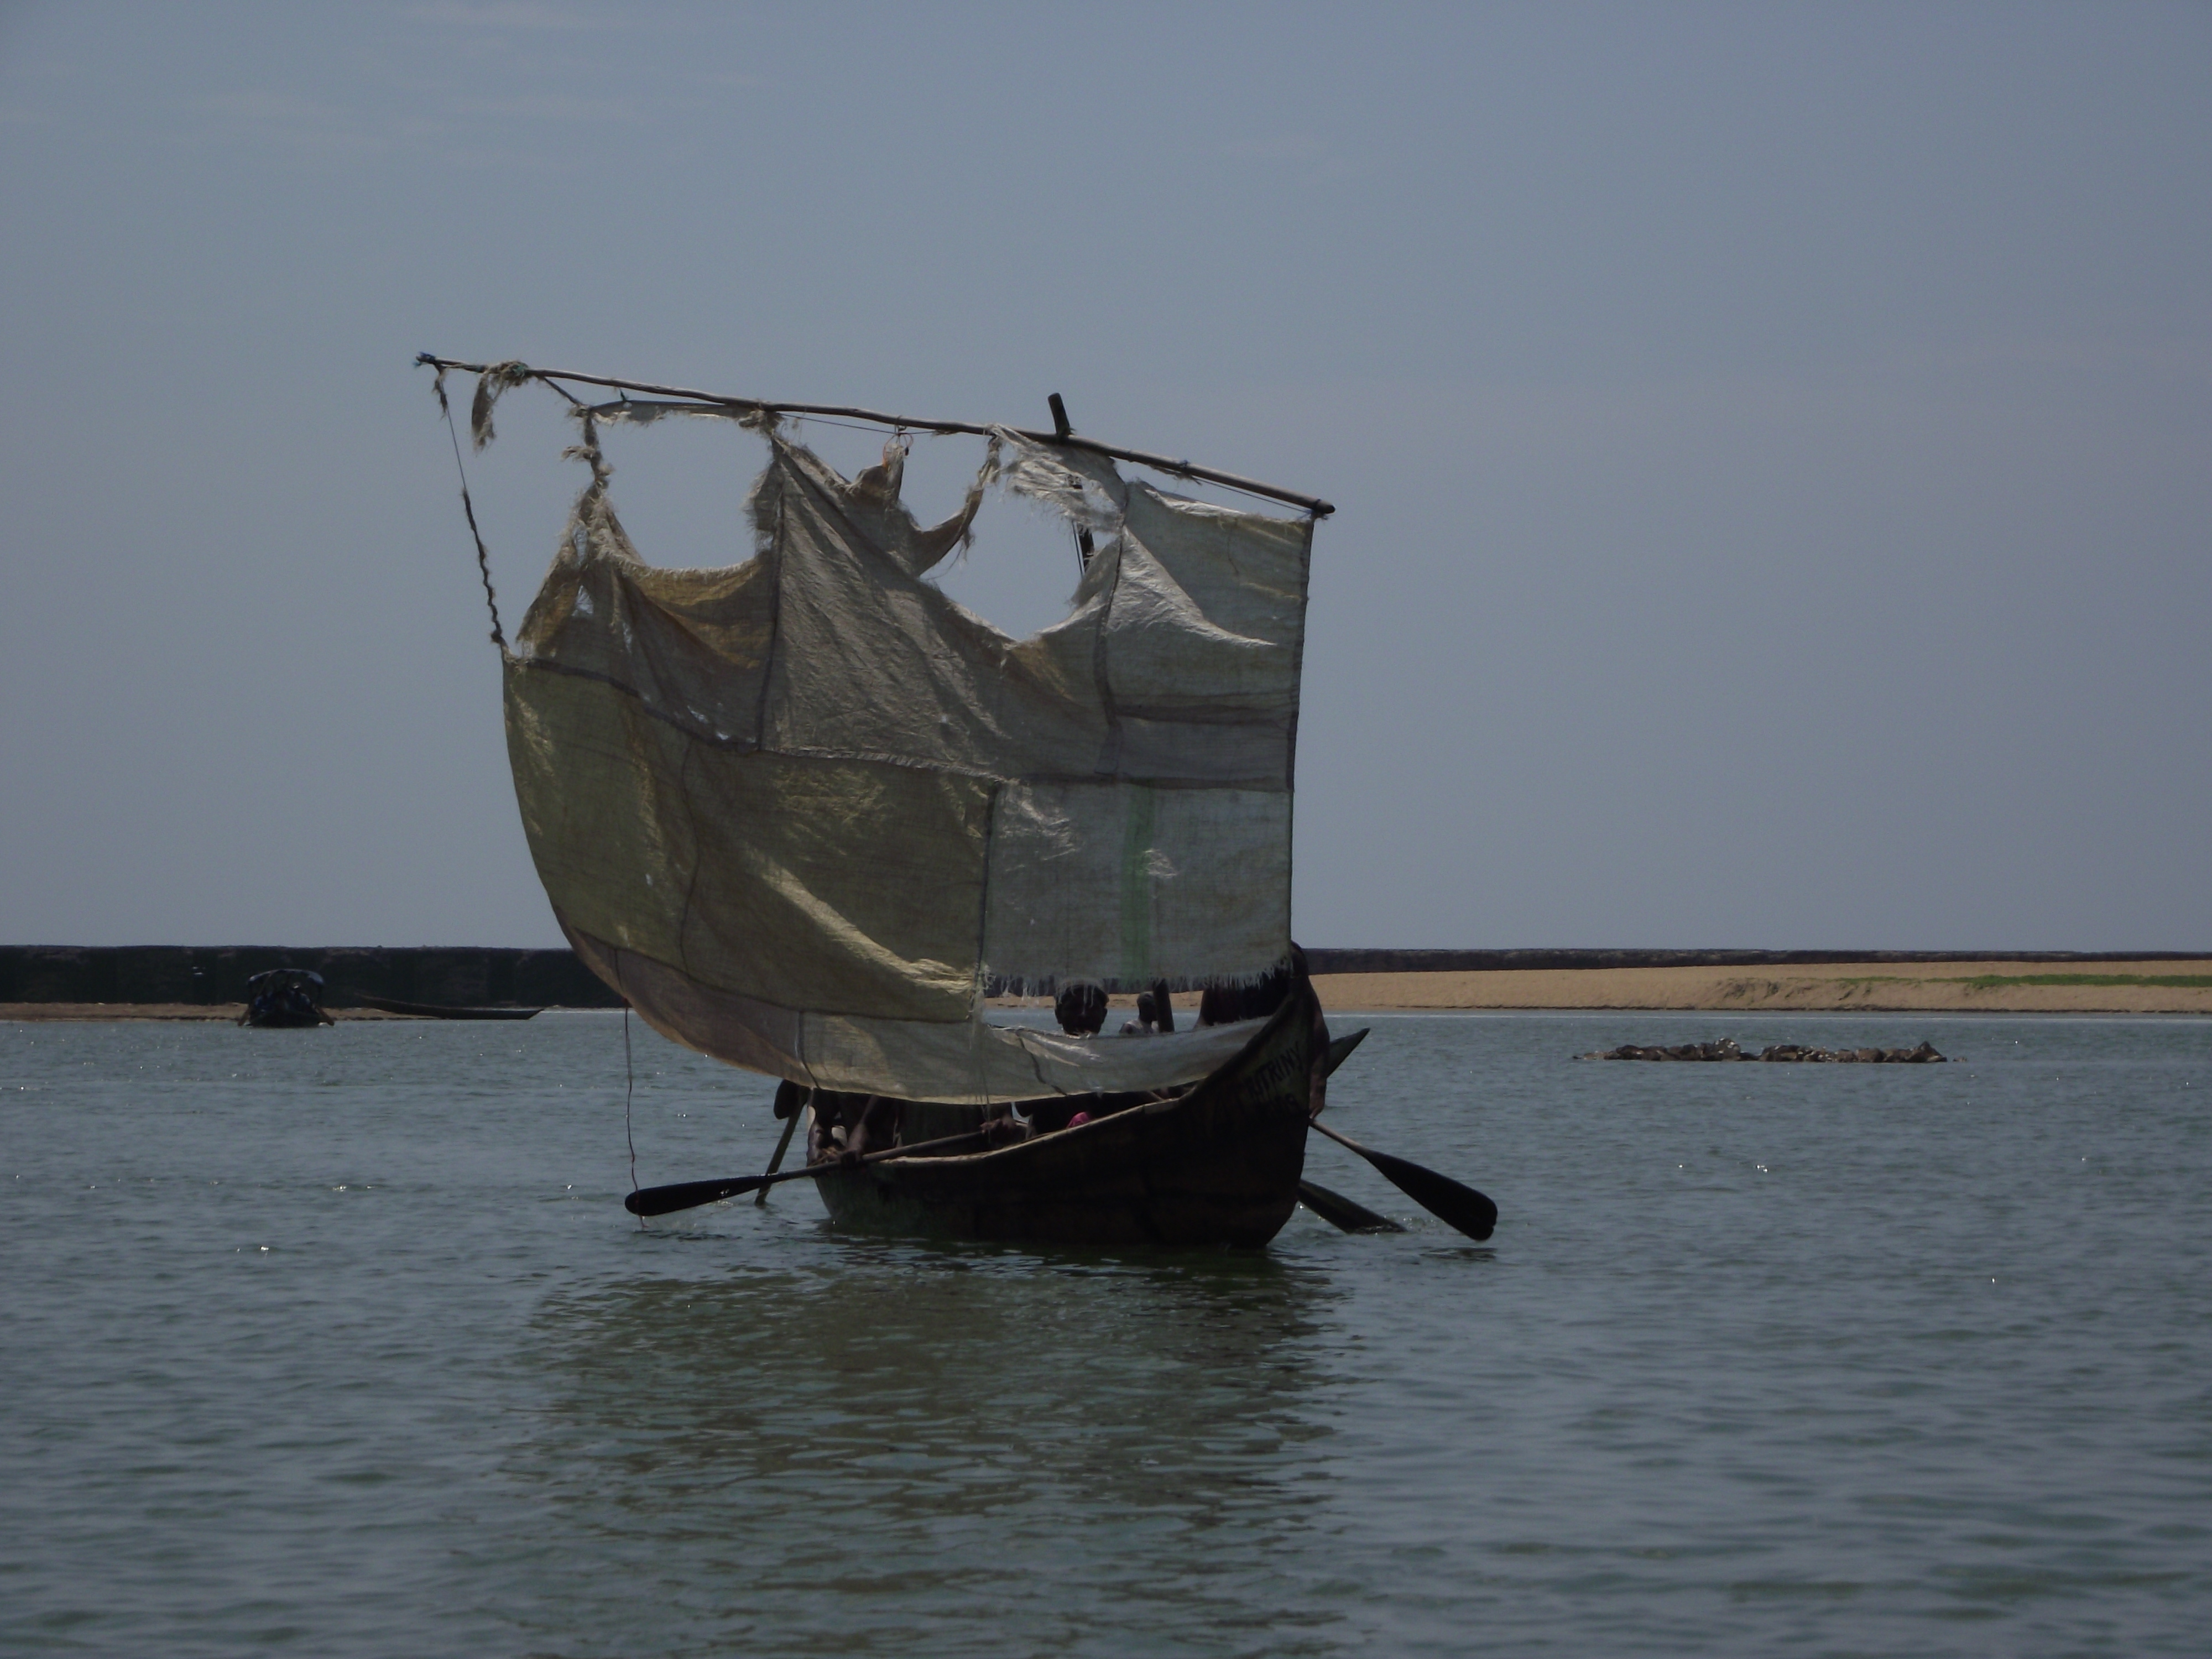
\includegraphics[width=5cm]{articles/Salut-vazaha/DSCF0211.JPG}
\smallbreak

\smallbreak
\hspace*{-0.65cm}
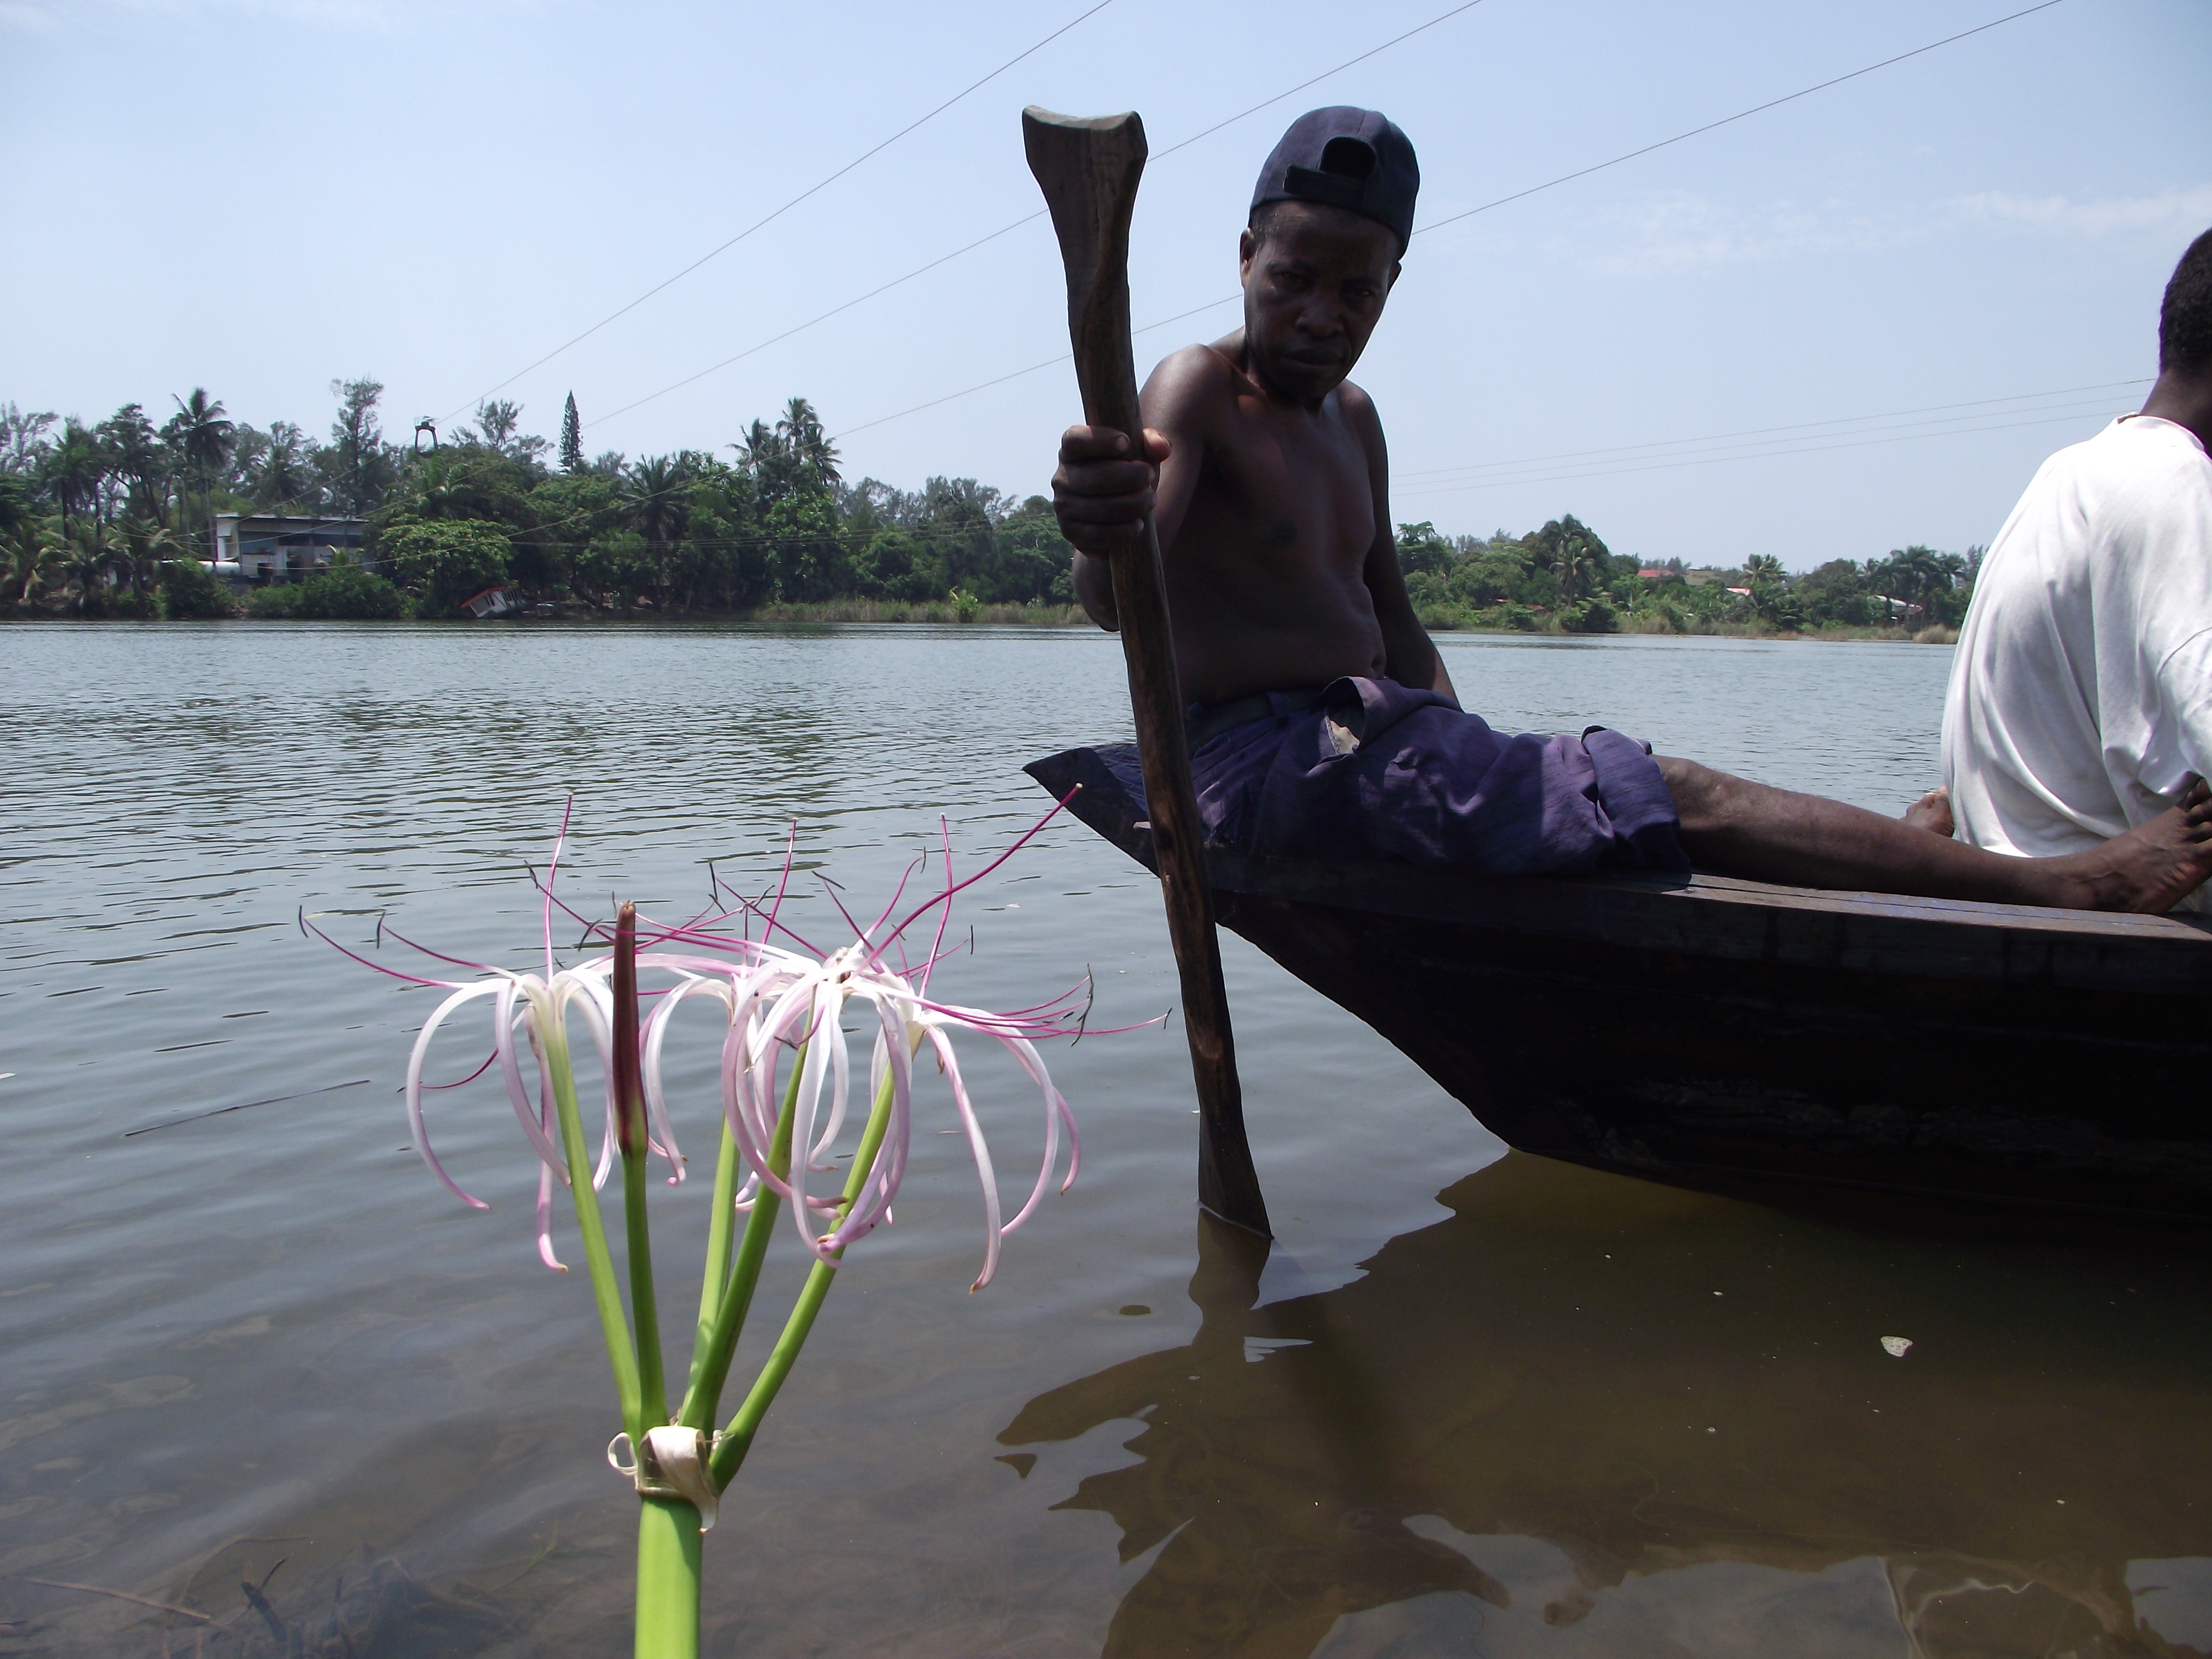
\includegraphics[width=5cm]{articles/Salut-vazaha/DSCF0225.JPG}
\smallbreak

Un petit tour du côté de la mer, là où rentrent les pêcheurs dans leur pirogue creusée dans un tronc d'arbre. C'est vraiment impressionnant de voir l'habileté qu'ont les pêcheurs pour fendre les vagues en essayant d'avoir le moins d'eau possible à rentrer dans la pirogue. Nous ne pourrions pas tenir plus de deux vagues avant que le bateau soit rempli, ici les pêcheurs vont et reviennent avec du poisson, et les jours se répètent.

\smallbreak
\hspace*{-0.65cm}
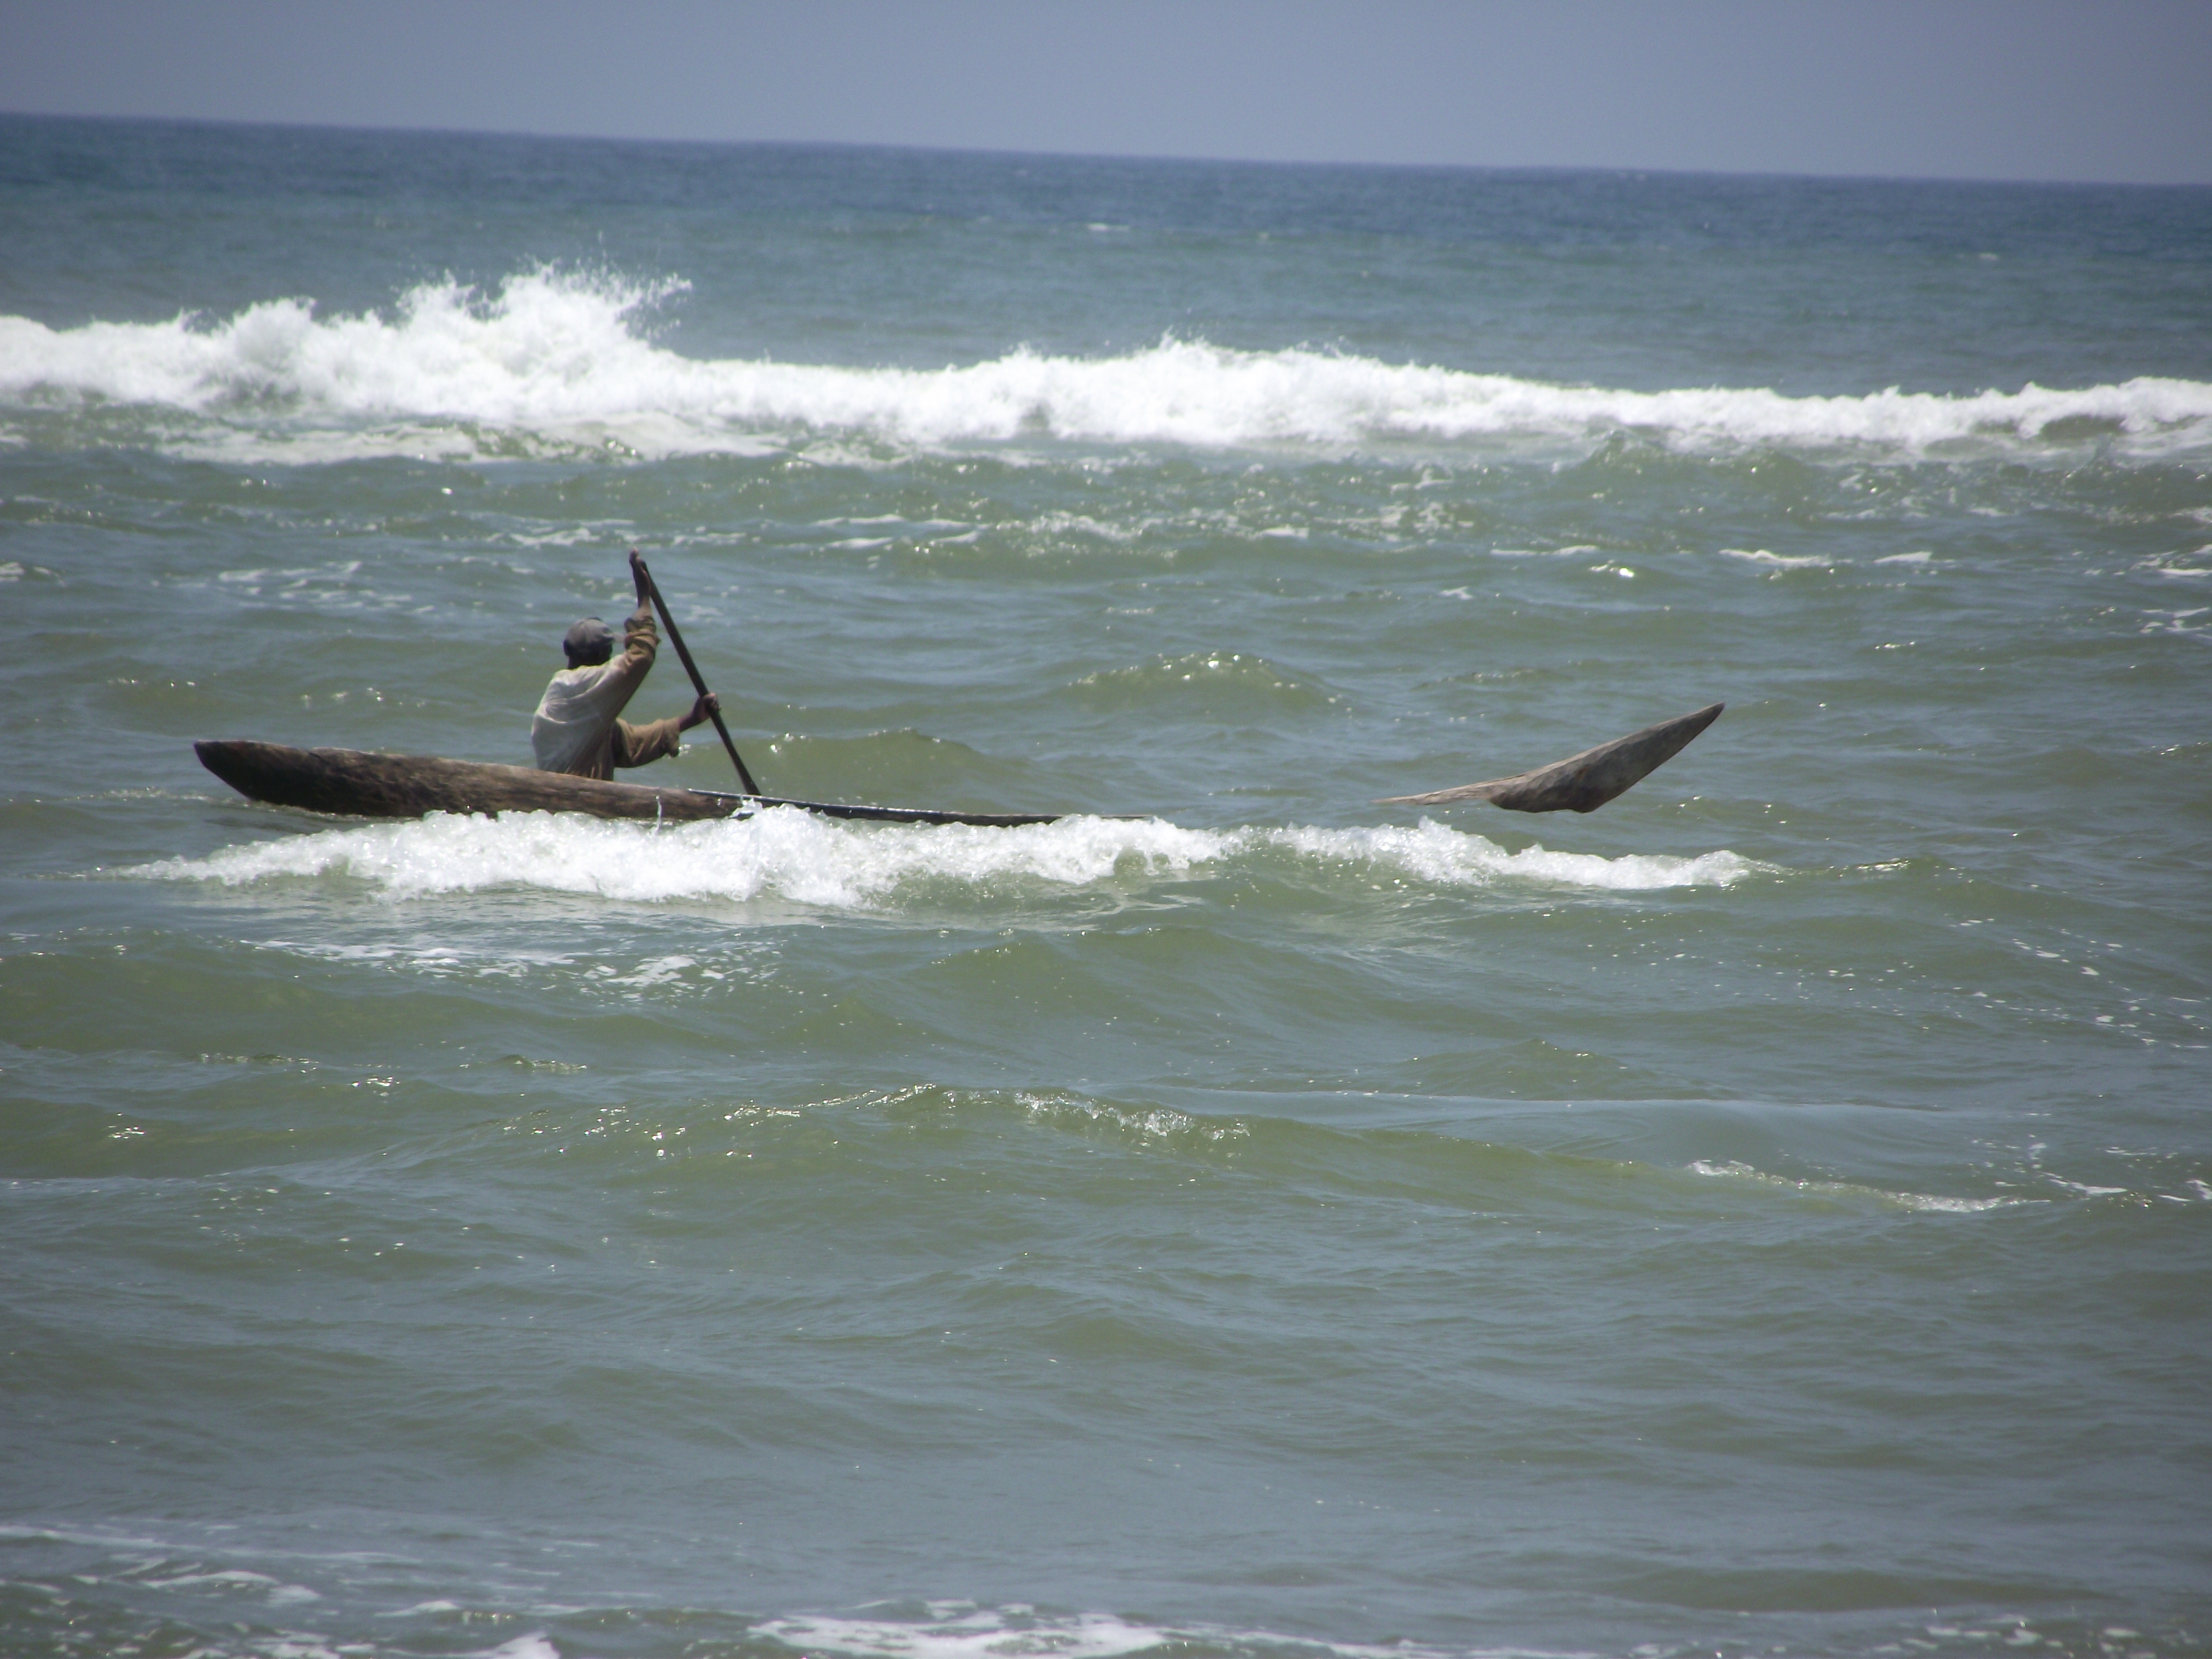
\includegraphics[width=5cm]{articles/Salut-vazaha/DSCF0241.JPG}
\smallbreak

Et puis c'est le départ de Manakar en taxi brousse pour aller à Ambalavao et visiter le petit parc d'Anja un peu plus au Sud. Je passe la nuit dans le taxi brousse avec un arrêt à Fianarantsoa vers 3 heures du matin, l'arrêt s'éternise, je me rendors dans le mini van arrêté et vers 5 heures on me réveille pour me dire de changer de taxi brousse, le transfert est fait, on part, super cet arrêt ça m'aura évité d'arriver à 4 heure à Ambalavao, du coup plus besoin de prendre une chambre pour finir la nuit, je vais directement au parc en profitant d'un groupe déjà formé et une guide super sympa. Je vais donc voir les lémuriens avec Delphine et Leo.

\smallbreak
\hspace*{-0.65cm}
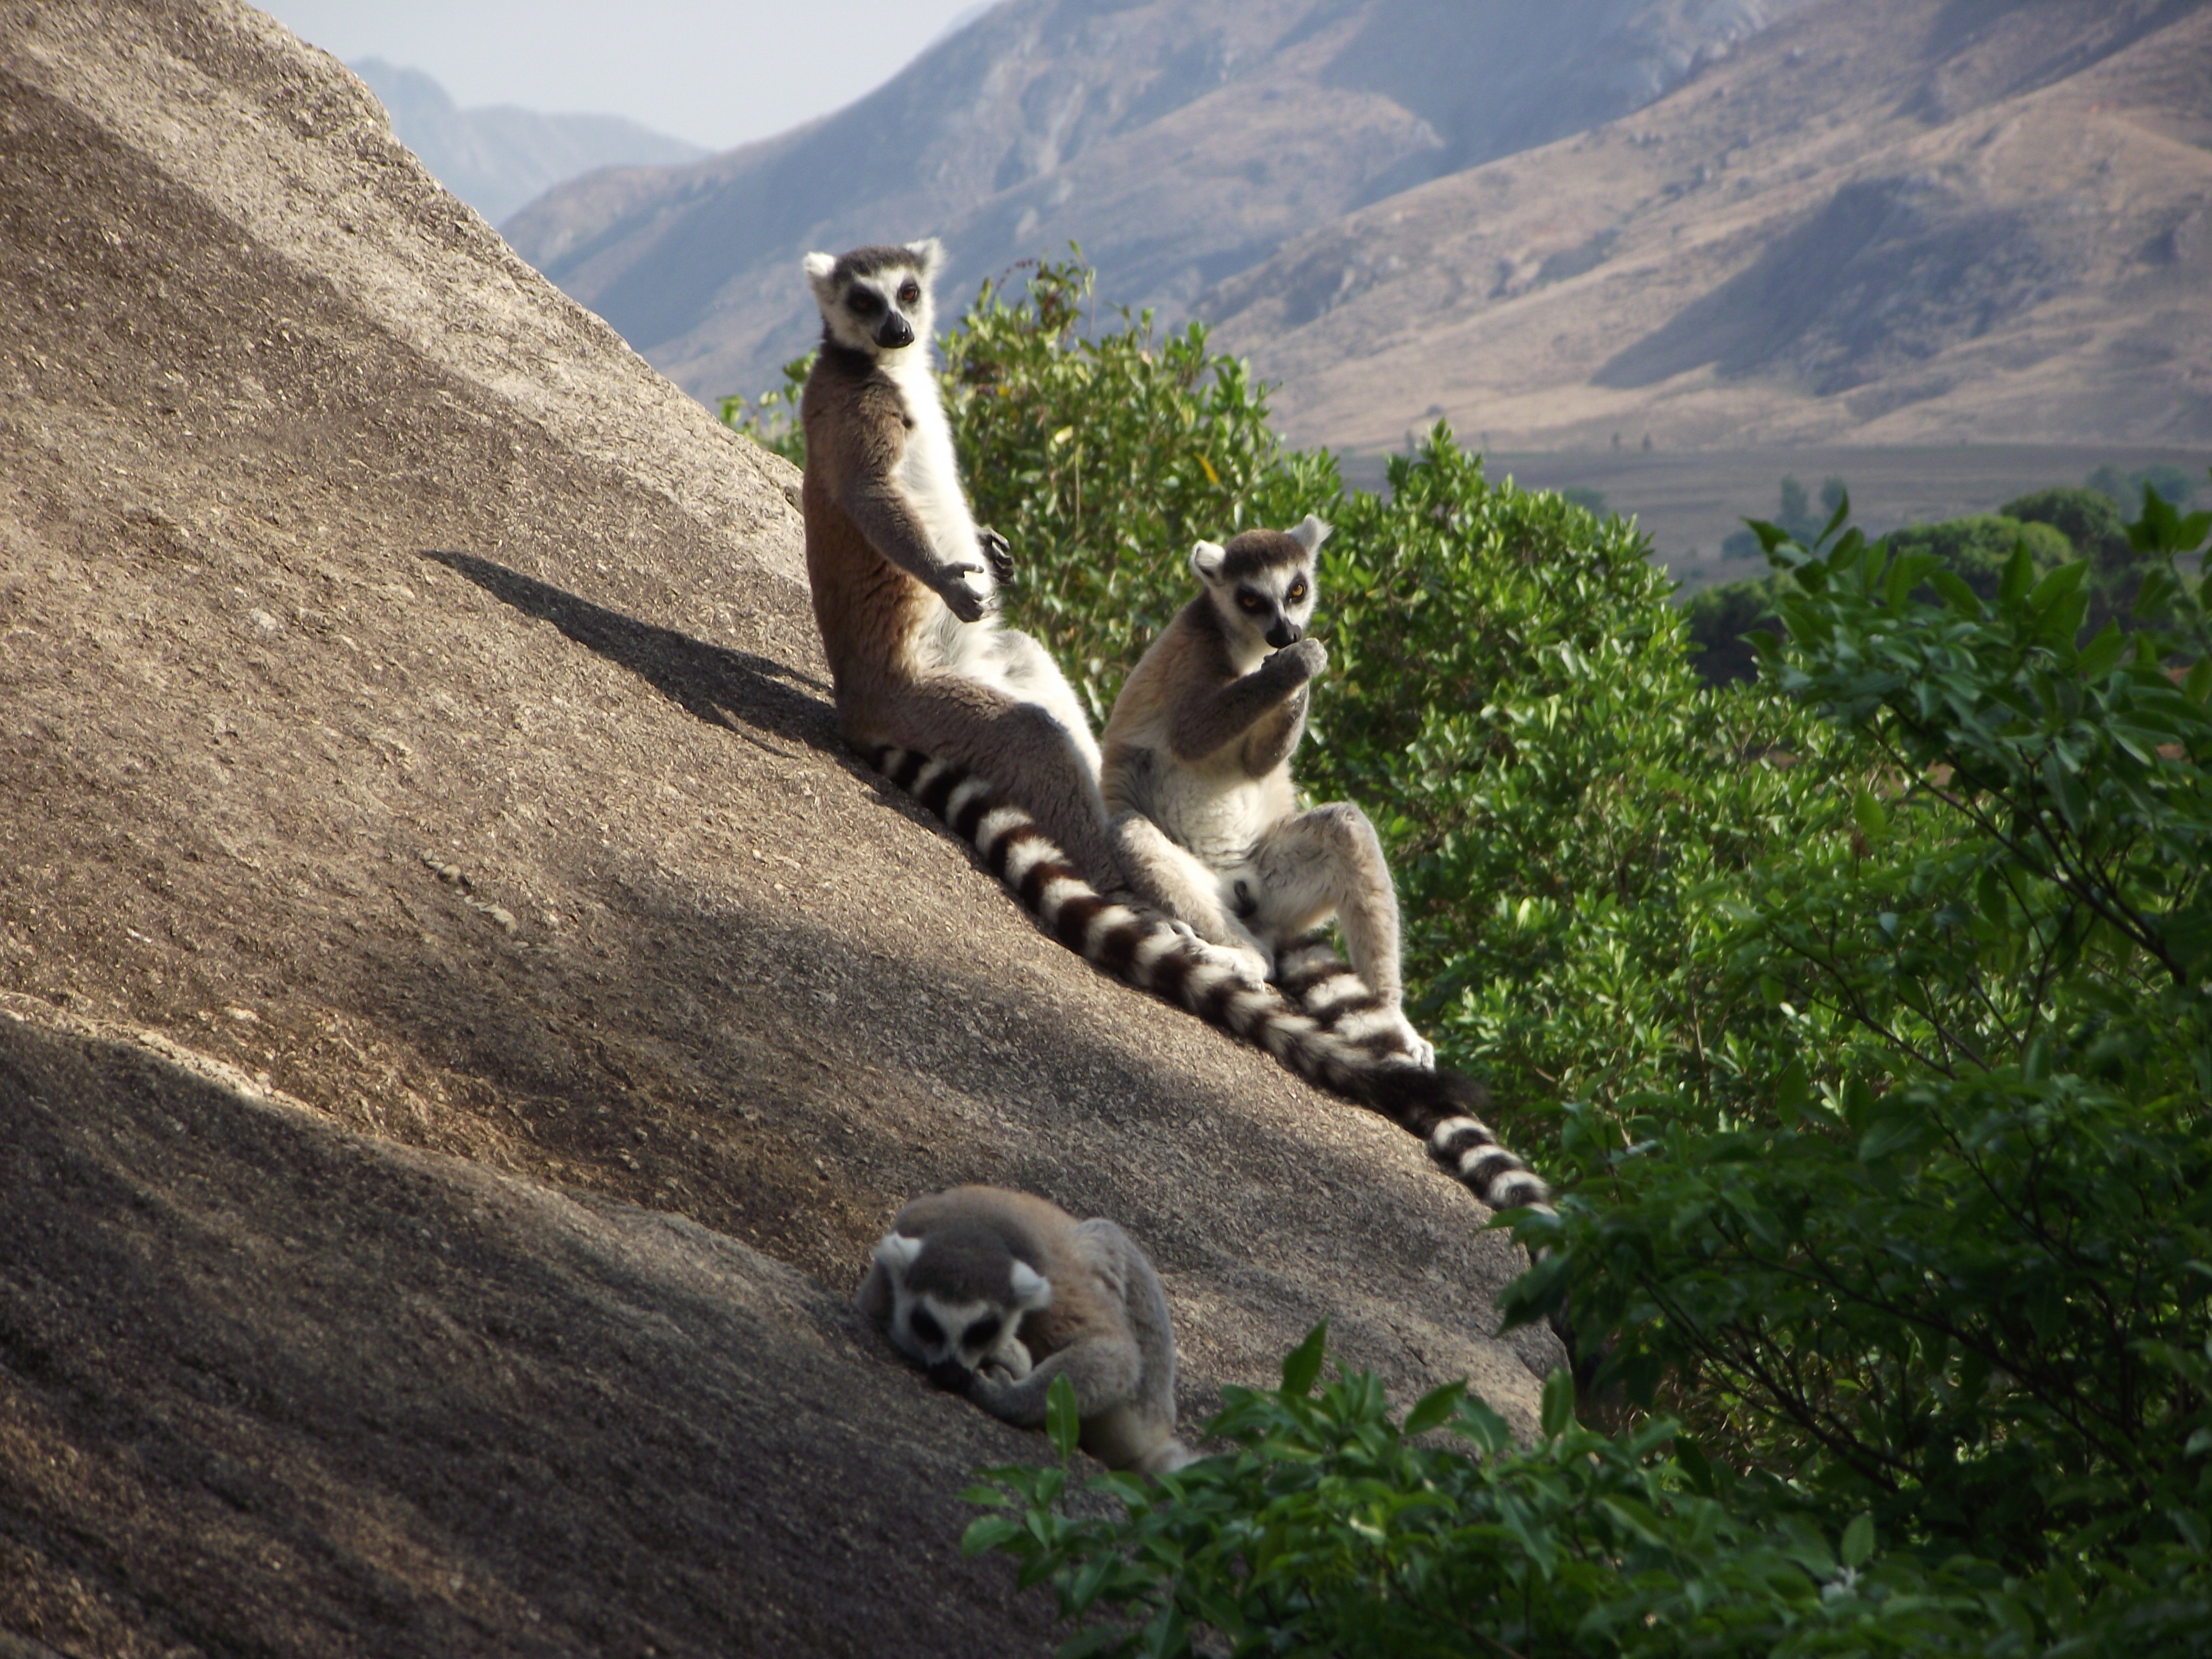
\includegraphics[width=5cm]{articles/Salut-vazaha/DSCF0262.JPG}
\smallbreak

Ici s'arrête ce reçit pour aujourd'hui. Je suis actuellement à Ranohira tout près d'un parc que je voulais visiter car il présente de très belles formations rocheuses, canons et piscine naturelle. Mais un autre élément est venu changer mes plans. J'ai rencontré Michel, un guide touristique qui rentre à Fort Dauphin prendre des clients et il me propose de faire le voyage avec lui pour un prix défiant toute concurrence, en effet le voyage est déjà payé par les touristes qu'il va chercher. Je vais donc aller à Fort Dauphin par la côte sud en deux journées de 4x4. Cette côte semble vraiment magnifique, je vous en dirais plus dans le prochain article..

A bientôt..

\end{multicols}

\bigskip
\textbf{\textsc{Commentaires}}

\medskip
Tatid a écrit le 21 nov. 2010 :
\begin{displayquote}
Eh bien mon salopard !!! Que de belles photos et que de belles aventures tout cela... Ça a l'air une fois de plus magique tes voyages comme ça "à la cool", avec à la clé, pas mal de rencontres sympa :-)
Je ne pensais plus à ton blog, quand hop, j'ai vu mon Google Reader qui affichait un petit (1) à côté du "Blog en vadrouille".
Allez, profite bien, prends-en plein les yeux, avant de rentrer à la capitale ;-)
\end{displayquote}

\medskip
Titou a écrit le 22 nov. 2010 :
\begin{displayquote}
Yeah pti Dud !
Eh bien te revoilà parti à l'autre bout du monde comme prévu ! Ça a l'air vraiment magnifique ce que tu vois et comme d'habitude tu fais de superbes rencontres ! Profites en à fond en faisant quand même gaffe à toi ! On suivra tes aventures comme toujours, même si nous on a pas un Google reader 2.0 version beta 12 codé en html qui nous dit que tu as laissé un message :p
(non ce commentaire ne vise personne en particulier :p)
aller enjoy and take care.
A plus ti Dud
biz
\end{displayquote}

\vfill

